%!TEX root = ../template.tex
%%%%%%%%%%%%%%%%%%%%%%%%%%%%%%%%%%%%%%%%%%%%%%%%%%%%%%%%%%%%%%%%%%%
%% chapter1.tex
%% NOVA thesis document file
%%
%% Chapter with introduction
%%%%%%%%%%%%%%%%%%%%%%%%%%%%%%%%%%%%%%%%%%%%%%%%%%%%%%%%%%%%%%%%%%%

\typeout{NT FILE chapter1.tex}%

\chapter{Introduction}
\label{cha:introduction}



\section{Motivation \& Problem Statement}
\label{sec:motivation+problem-statement}
\subsection{Breast Cancer - A Global Health Challenge}
\gls{BC} is currently one of the biggest public health challenges worldwide. In 2022, 
more than $2.3$ million new cases of \gls{BC} were diagnosed, resulting in around $665,\!000$ global deaths 
\cite{bcaData2024_bray} (Bray \textit{et al.}, 2024). Other studies estimate that \gls{BC} will continue to not only be 
the most commonly diagnosed cancer but also to increase in incidence, with projections indicating that by 2040, the number 
of deaths will almost double and the number of new cases will be around $3.2$ million \cite{bca_data_Arnold2022Current} 
(Arnold \textit{et al.}, 2022). These figures underline the high incidence and mortality 
associated with the disease, highlighting the ongoing need to develop more effective strategies for its diagnosis 
and treatment.

% \begin{table}[htbp]
% \centering
% \caption{Breast cancer incidence (new cases) and mortality (deaths) in 2020 by age at diagnosis, world region and Human Development Index level.\cite{bca_data_Arnold2022Current} (Arnold \textit{et al.}, 2022).}
% \label{tab:breast_cancer_incidence}
% \scriptsize
% \begin{tabular}{|l|r|r|r|r|r|r|r|}
% \hline
% \textbf{POPULATION\textsuperscript{a} (in millions)} & \multicolumn{2}{c|}{\textbf{$<$50 years}} & \multicolumn{2}{c|}{\textbf{50+ years}} & \multicolumn{3}{c|}{\textbf{NEW CASES}} \\
% \cline{2-8}
% \textbf{} & \textbf{N} & \textbf{(\%)} & \textbf{N} & \textbf{(\%)} & \textbf{N ($<$50 years)} & \textbf{(\%)} & \textbf{ASR N (50+ years)} \\
% \hline
% Eastern Africa & 201.6 & 7.0 & 22.8 & 2.3 & 22,801 & 3.4 & 22,908 \\
% Middle Africa & 81.4 & 2.8 & 8.6 & 0.9 & 10,272 & 1.5 & 7,624 \\
% Northern Africa & 100.9 & 3.5 & 21.6 & 2.2 & 25,496 & 3.8 & 31,632 \\
% Southern Africa & 28.1 & 1.0 & 6.1 & 0.6 & 5,680 & 0.9 & 10,846 \\
% Western Africa & 179.1 & 6.2 & 20.4 & 2.1 & 21,973 & 3.3 & 27,366 \\
% Caribbean & 15.9 & 0.6 & 6.1 & 0.6 & 4,044 & 0.6 & 10,668 \\
% Central America & 72.2 & 2.5 & 19.4 & 2.0 & 14,524 & 2.2 & 24,392 \\
% South America & 161.6 & 5.6 & 57.1 & 5.8 & 45,596 & 6.9 & 110,876 \\
% Northern America & 116.6 & 4.0 & 69.7 & 7.1 & 52,224 & 7.8 & 229,367 \\
% Eastern Asia & 528.6 & 18.4 & 294.0 & 29.9 & 177,693 & 26.7 & 373,943 \\
% All but China & 64.9 & 2.3 & 52.2 & 5.3 & 37,427 & 5.6 & 97,838 \\
% China & 463.7 & 16.1 & 241.8 & 24.6 & 140,266 & 21.1 & 276,105 \\
% South-Eastern Asia & 257.0 & 8.9 & 77.7 & 7.9 & 55,090 & 8.3 & 103,849 \\
% South Central Asia & 791.1 & 27.5 & 186.0 & 18.9 & 94,730 & 14.2 & 160,151 \\
% All but India & 262.1 & 9.1 & 52.2 & 5.3 & 27,621 & 4.2 & 48,899 \\
% India & 529.0 & 18.4 & 133.9 & 13.6 & 67,109 & 10.1 & 111,252 \\
% Western Asia & 108.1 & 3.8 & 24.5 & 2.5 & 24,738 & 3.7 & 35,977 \\
% Central-Eastern Europe & 91.8 & 3.2 & 63.4 & 6.4 & 33,883 & 5.1 & 124,825 \\
% Northern Europe & 32.4 & 1.1 & 21.4 & 2.2 & 14,755 & 2.2 & 68,422 \\
% Southern Europe & 43.0 & 1.5 & 35.4 & 3.6 & 25,359 & 3.8 & 94,826 \\
% Western Europe & 55.7 & 1.9 & 44.1 & 4.5 & 30,668 & 4.6 & 138,348 \\
% Australia/New Zealand & 9.9 & 0.3 & 5.4 & 0.5 & 4,844 & 0.7 & 18,433 \\
% Melanesia & 4.7 & 0.2 & 0.8 & 0.1 & 1,022 & 0.2 & 1,193 \\
% Micronesia/Polynesia & 0.5 & 0.0 & 0.1 & 0.0 & 116 & 0.0 & 265 \\
% Low HDI & 443.6 & 15.4 & 50.9 & 5.2 & 52,691 & 7.9 & 56,881 \\
% Medium HDI & 924.6 & 32.1 & 211.4 & 21.5 & 115,253 & 17.3 & 192,405 \\
% High HDI & 1025.5 & 35.6 & 416.5 & 42.3 & 280,414 & 42.1 & 545,024 \\
% Very high HDI & 485.5 & 16.9 & 305.3 & 31.0 & 216,804 & 32.6 & 800,655 \\
% \textbf{World} & \textbf{2880.3} & \textbf{100} & \textbf{984.5} & \textbf{100} & \textbf{665,508} & \textbf{100} & \textbf{1,595,911} \\
% \hline
% \end{tabular}
% \end{table}

% \begin{figure}[h!]
%     \centering
%     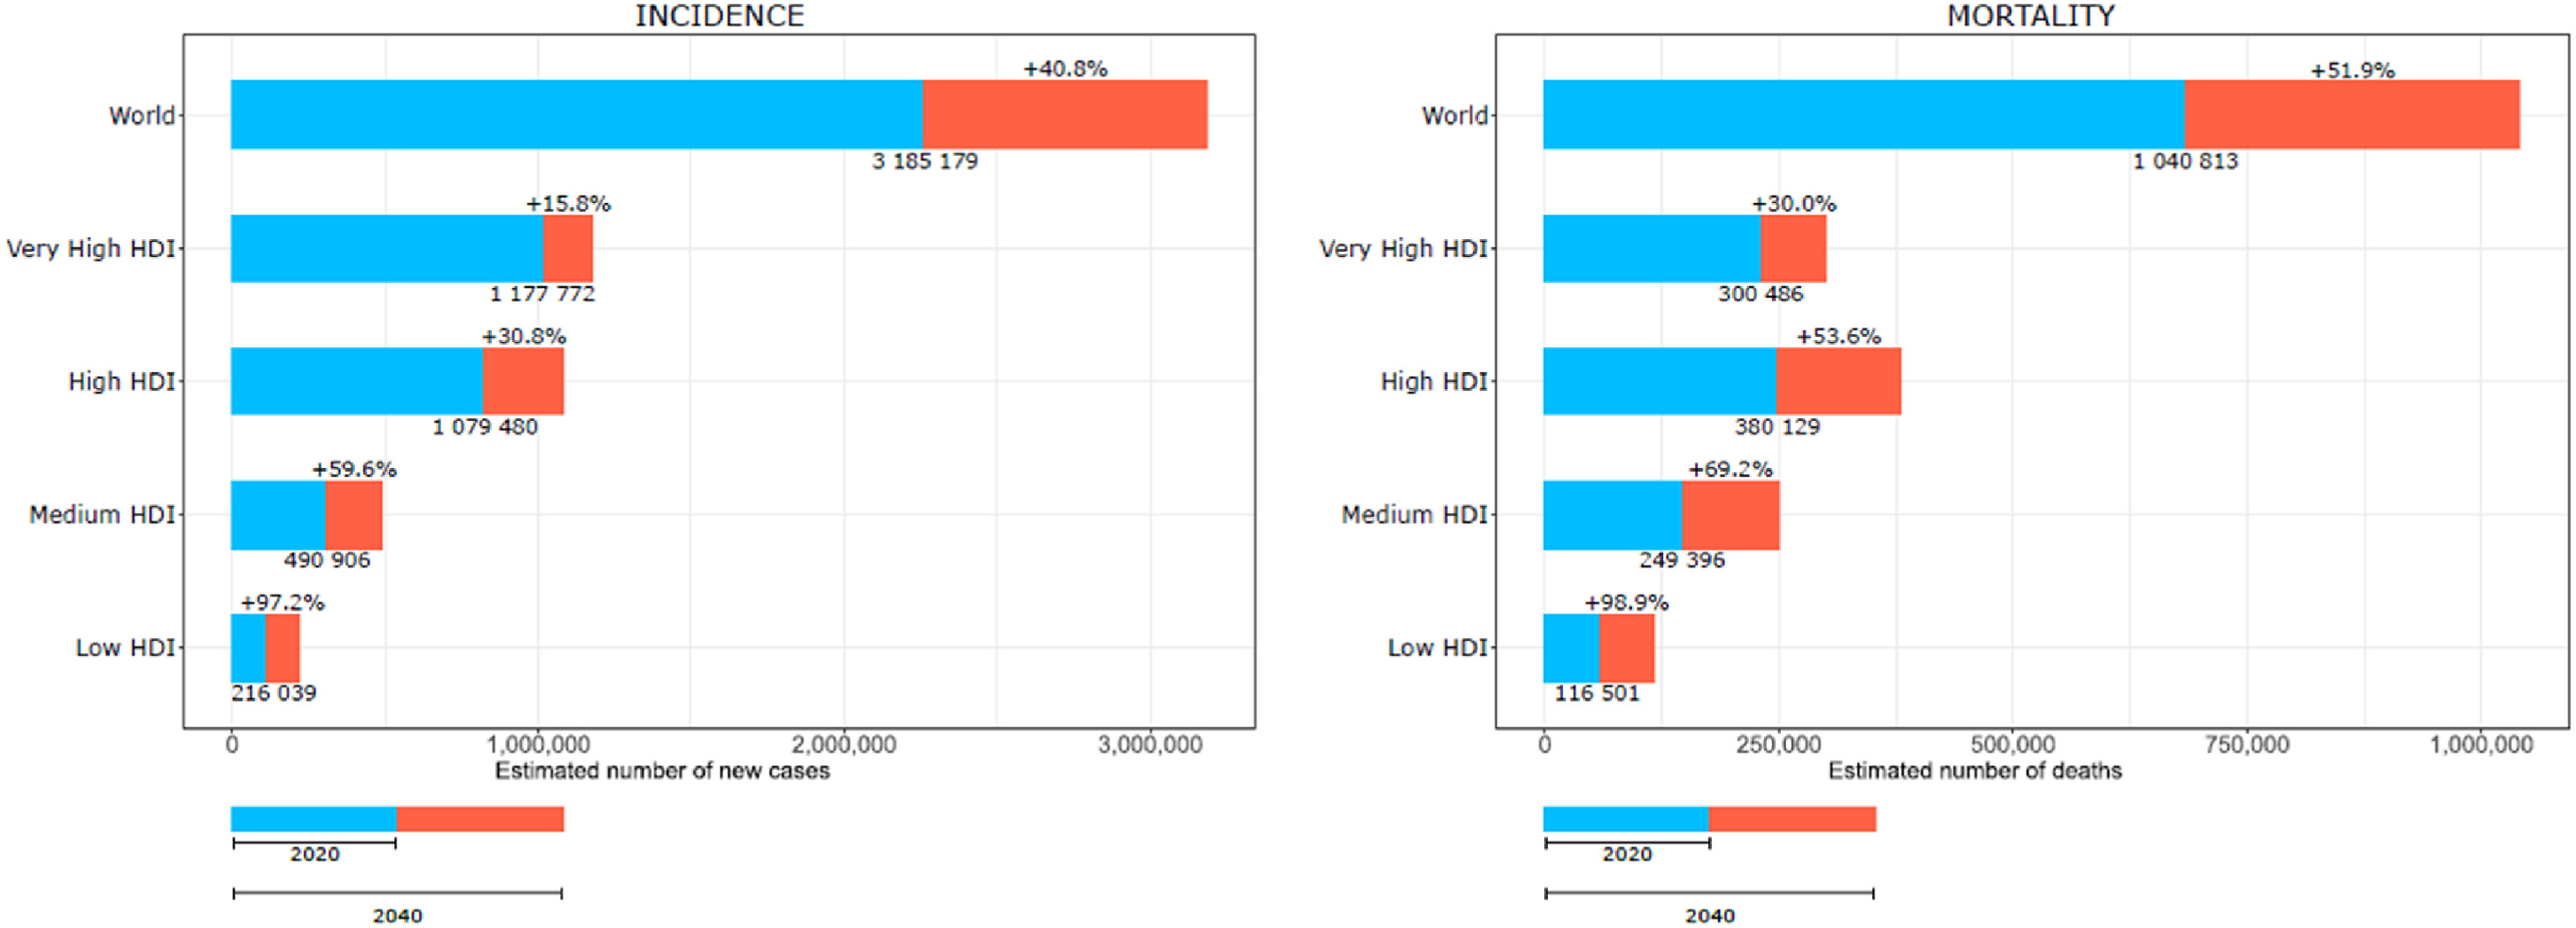
\includegraphics[width=\textwidth]{BC2020-2040.jpg} % Caminho para sua imagem
%     \caption{Projected changes in breast cancer incidence and mortality between 2020 and 2040 across Human Development 
%     Index (HDI) categories. \cite{bca_data_Arnold2022Current}}
%     \label{fig:bc_incidence_mortality}
% \end{figure}

%% Incidencia de cancro -> converter imagem em código LaTeX https://gco.iarc.who.int/media/globocan/factsheets/populations/900-world-fact-sheet.pdf

BC is characterized by marked biological heterogeneity, manifested in multiple molecular subtypes that exhibit distinct 
clinical behaviors \cite{bc_molecular_Perou2000} (Perou \textit{et al.}, 2000). Each subtype exhibits substantial differences in 
terms of tumor aggressiveness, metastatic potential, and behavior to specific therapies 
\cite{bc_subtypes_Prat2015Clinical} (Prat \textit{et al.}, 2015). Thus, accurate classification of these subtypes is essential 
to enable personalized therapeutic approaches, with a direct impact on treatment efficacy and patient prognosis. 
\cite{need_for_subtype_treatments_Testa2020Breast} (Testa \textit{et al.}, 2020).

\subsection{Can we improve the classification of Breast Cancer subtypes?}
Among the emerging candidates for robust biomarkers for the classification of  \gls{BC} subtypes are \gls{miRNAs}, 
small non-coding RNA molecules that play a crucial regulatory role in gene expression. They are estimated to 
modulate the expression of about one-third of the genes in the human genome \cite{mirna_importance_Hammond2015An} 
(Hammond \textit{et al.}, 2015) and are implicated in the regulation of multiple physiological and pathological 
processes, including various human diseases \cite{mirna_as_biomarkers_Ho2022} (Ho \textit{et al.}, 2022).

Given their regulatory nature, several studies have demonstrated a significant association between \gls{miRNAs} expression 
profiles and relevant clinical characteristics in the context of \gls{BC}, including processes such as tumor 
progression and metastasis development \cite{mirna_as_biomarkers_Ho2022} \cite{mirnas_in_bc_Muñoz2023} (Muñoz \textit{et al.}, 2023) 
\cite{mirna_as_bio_for_sub_Blenkiron2007MicroRNA} (Blenkiron \textit{et al.}, 2007). 
In addition to these aspects, a seminal 
study by Blenkiron \textit{et al.} (2007) demonstrated that \gls{miRNAs} expression profiles can effectively distinguish between 
different molecular subtypes of \gls{BC}, highlighting their potential as a precise subtyping tool. This ability to 
discriminate between subtypes reinforces the value of \gls{miRNAs} as promising clinical biomarkers.

\subsection{How to identify the most relevant miRNAs?}

The identification of the most relevant \gls{miRNAs} for \gls{BC} subtyping represents a major analytical challenge due 
to the complexity of these high dimensional regulatory molecules, non-linearity interactions between and 
clinical phenotypes require advanced computational approaches to be effectively modelled. Recent advances in \gls{AI}, 
particularly in \gls{ML} and \gls{DL}, have demonstrated remarkable potential in extracting meaningful patterns from 
high-dimensional and heterogeneous (data from distinct nature) biomedical data. These approaches enable not only the 
accurate classification of \gls{BC} subtypes but also the identification of discriminative \gls{miRNAs} signatures, 
supporting their integration as actionable biomarkers in clinical workflows.

In this context, \gls{ML} and \gls{DL} models are particularly well suited for the task of robustly characterizing and 
explaining the profiles of \gls{miRNAs}-based biomarkers — should such biomarkers exist — with the potential to effectively 
discriminate between different \gls{BC} subtypes, as already seen in a study done by  \cite{ml_gastric_Azari2023} Azari \textit{et al.} 2023 where \gls{ML} 
algorithms identified potential diagnostic and prognostic \glossary{miRNAs} in gastric cancer, showing high accuracy in the 
identification of reliable biomarkers for this disease.

This reality reinforces the urgency of developing advanced computational tools that can enable more precise molecular 
characterization and guide personalized therapeutic decisions, ultimately improving clinical outcomes for patients with 
aggressive and hard-to-treat \gls{BC} subtypes.

\section{Background}
\label{sec:background}
\subsection{Biology}

The modern understanding of how genetic information is stored, interpreted, and regulated in cells is based on a fundamental 
principle known as the Central Dogma of Molecular Biology. This concept, first formulated by Francis Crick in $1958$, describes 
the unidirectional flow of genetic information in cells: from deoxyribonucleic acid (DNA) to ribonucleic acid (RNA), and from there 
to protein synthesis. According to this model, genes encoded in DNA are transcribed into messenger RNA (mRNA), which in turn is 
translated into proteins—the functional molecules responsible for most essential biological processes. This dogma has served as 
the basis for much of the research in molecular biology and biotechnology.

However, in recent decades, it has become clear that this flow of information is regulated in a much more complex way than initially 
thought. In particular, it has been discovered that a substantial part of the genome is transcribed into non-coding RNA, i.e., RNA 
that does not give rise to proteins but plays fundamental regulatory roles. It is in this context that microRNAs (miRNAs) emerge, 
small RNA molecules with central functions in the regulation of gene expression. Their discovery has broadened the classical view 
of the central dogma, introducing new layers of post-transcriptional control that decisively influence normal and pathological biological phenomena.

\subsubsection*{DNA \& RNA - the Genetic Code}

At the molecular level, the genetic information of all living organisms is encoded in a molecule called deoxyribonucleic acid (DNA). 
DNA consists of two complementary strands arranged in a double helix structure, with each strand consisting of a sequence of nucleotides. 
These nucleotides are composed of a sugar-phosphate structure and one of four nitrogenous bases: adenine (A), cytosine (C), guanine (G), 
and thymine (T) \cite{ConceptsBiology_DNA}. When in the helix structure, these bases can only be linked to their corresponding base: 
adenine can only be linked to thymine and cytosine to guanine, and it is in the sequence of bases that the instructions necessary for the 
synthesis of all the proteins that govern cell structure and function are encoded.
 
\begin{figure}[h]
\centering
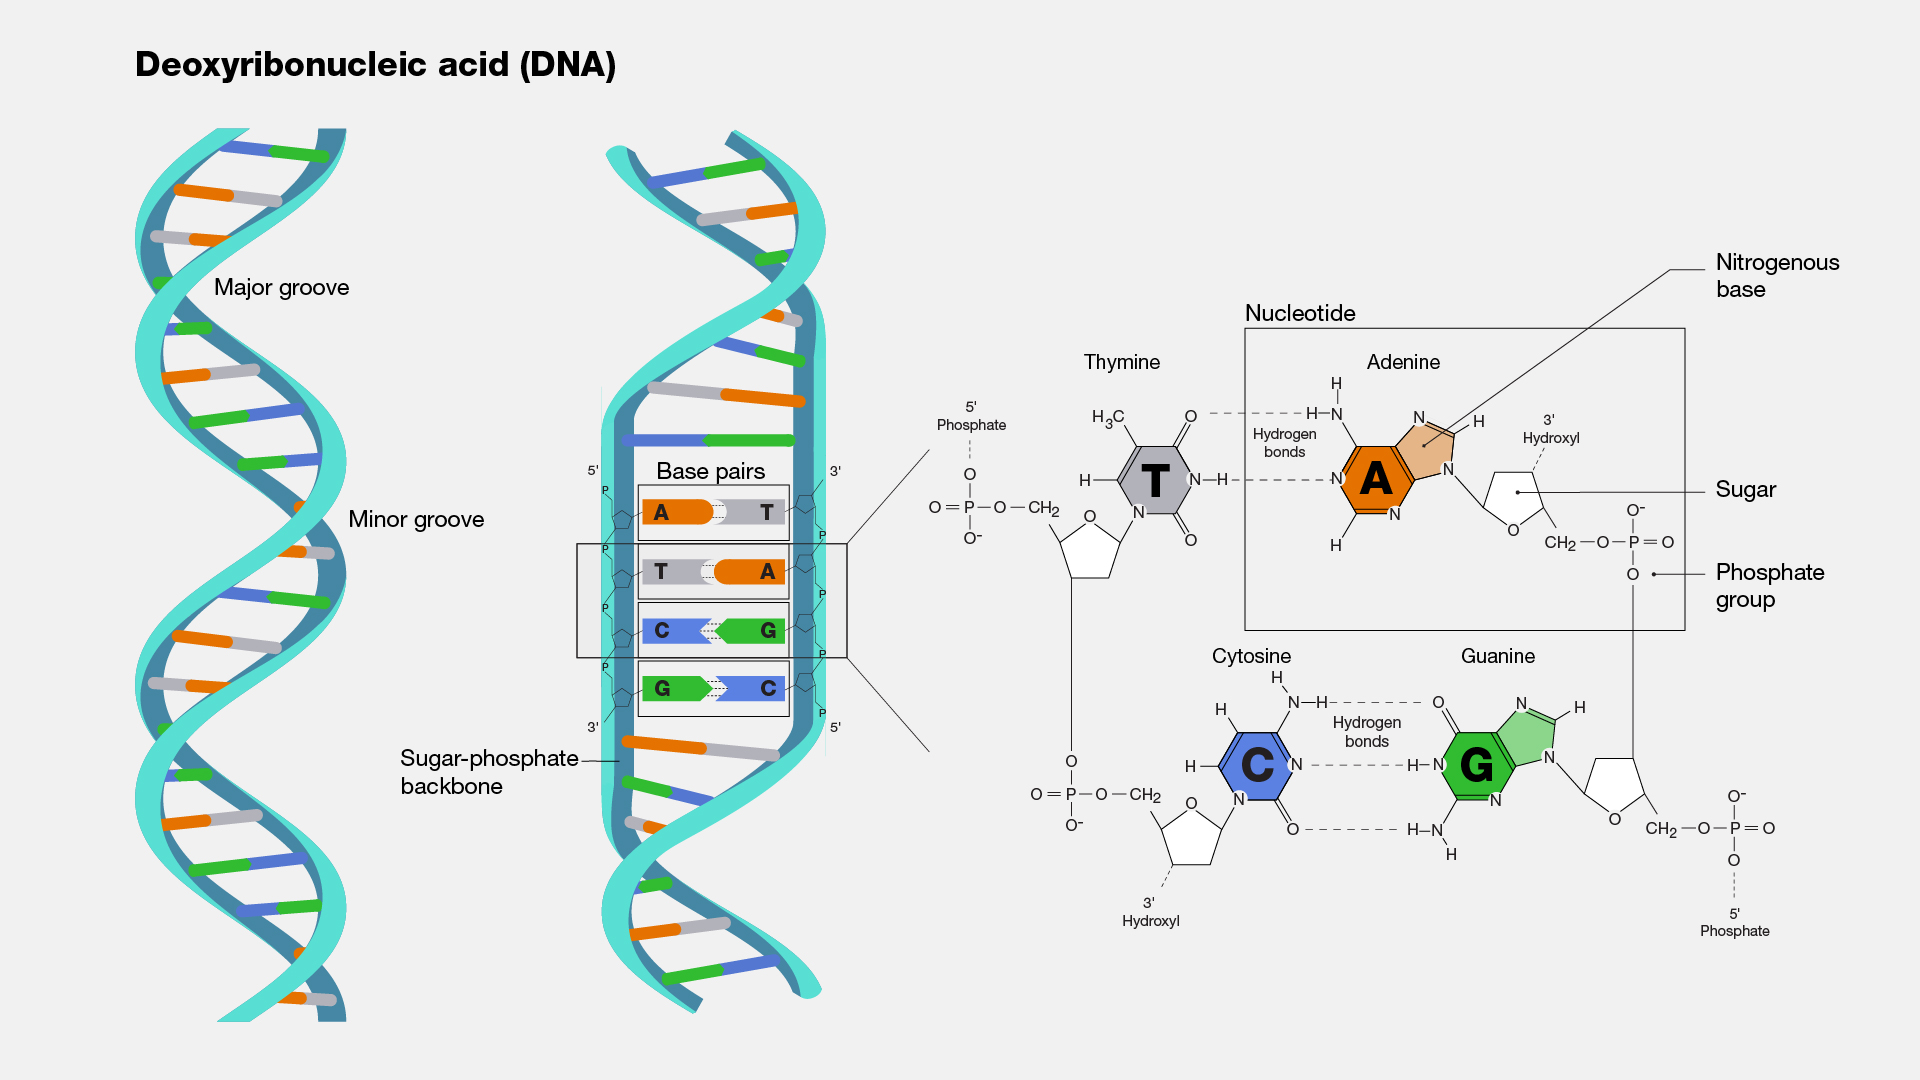
\includegraphics[width=0.6\textwidth]{dna.jpg}
\caption{Structure of the DNA double helix}
\label{fig:dna}
\end{figure}

The functional units of DNA are called genes, which are discrete sequences that contain the instructions for producing proteins. However, 
DNA itself cannot participate directly in protein synthesis. Instead, a process called transcription is used to copy the information 
from a gene to a ribonucleic acid (RNA) molecule \cite{basic_biology_NCBI2002}. Unlike DNA, RNA is single-stranded and uses uracil (U) 
instead of thymine as one of its bases.

Among the various types of RNA, the best known is messenger RNA (mRNA), which serves as an intermediary between genes and proteins. 
During transcription, an mRNA molecule is synthesized as a complementary copy of a gene, and this mRNA carries the genetic message 
from the DNA in the nucleus to the ribosomes in the cytoplasm, where protein synthesis occurs. This process, known as translation, 
is where the mRNA sequence is read in triplets (called codons), each of which corresponds to a specific amino acid \cite{central_dogma_molecular}.

%melhorar estrutura da imagem para ser como no paper
\begin{figure}[h]
\centering
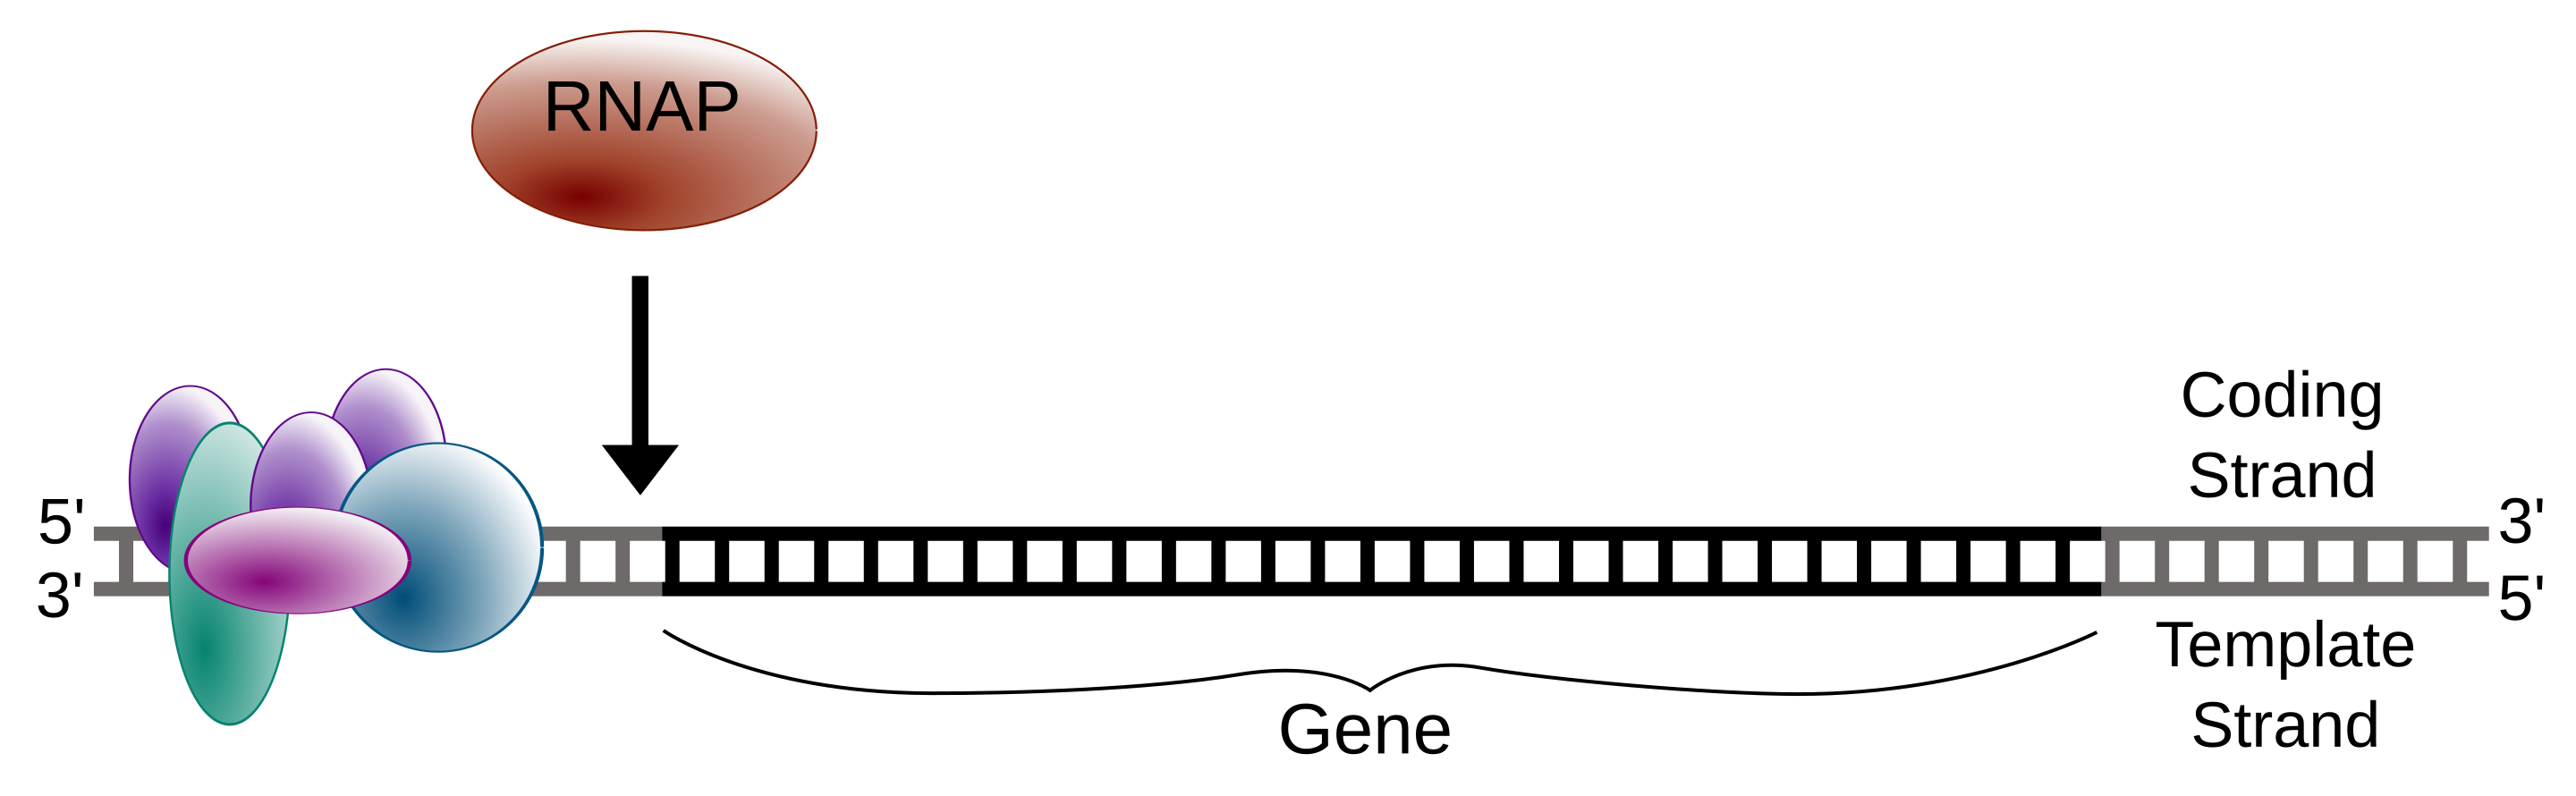
\includegraphics[width=0.3\textwidth]{transcription1.png}

\includegraphics[width=0.3\textwidth]{transcription2.png}
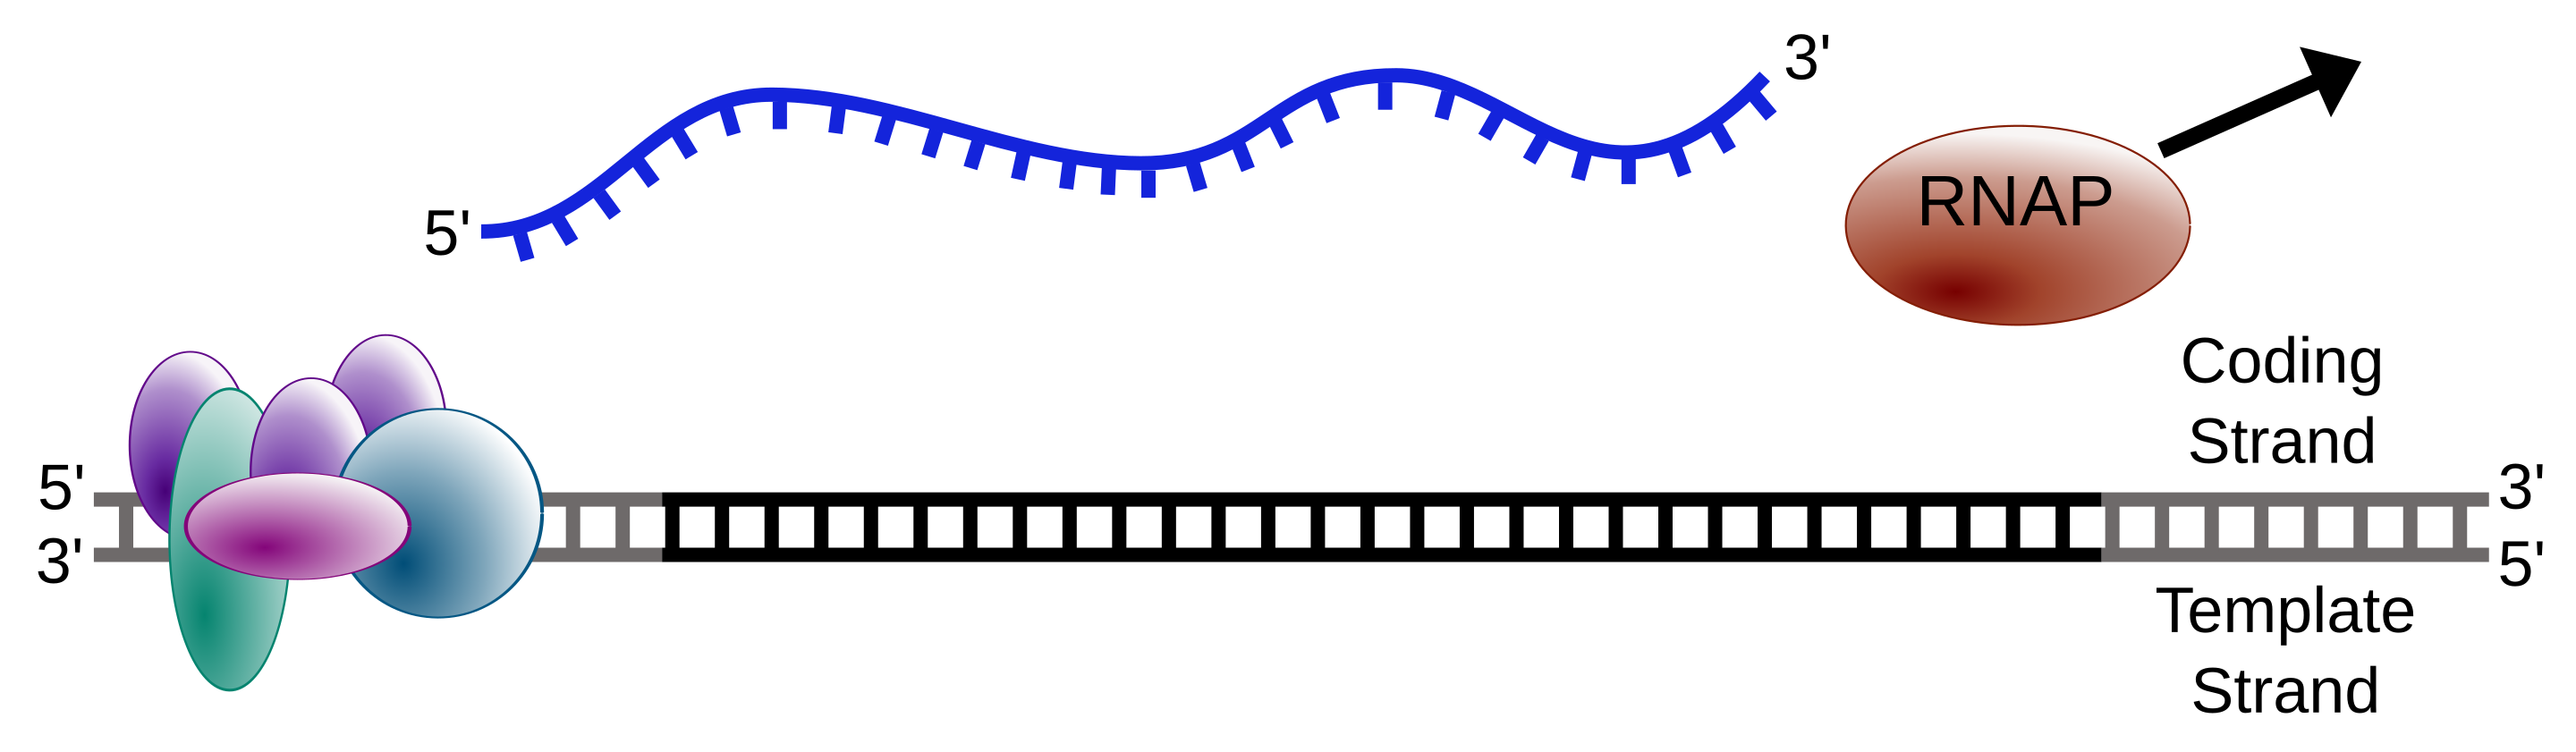
\includegraphics[width=0.3\textwidth]{transcription3.png}
\caption{Illustration of the transcription mechanism: (a) initiation, (b) elongation, and (c) termination}
\label{fig:transcription}
\end{figure}

The set of rules by which the nucleotide sequence in messenger RNA is translated into a sequence of amino acids is known as 
the genetic code. This code is composed of triplets of nucleotides, called codons, where each codon specifies one of the twenty 
standard amino acids used in protein synthesis \cite{genetic_codeNovozhilov2008O}.

The genetic code is described as redundant but unambiguous. Redundancy means that most amino acids are encoded by more than 
one codon—for example, leucine is specified by six different codons—which provides a certain degree of robustness to the system. 
At the same time, the code is unambiguous because each codon corresponds to only one amino acid; that is, a given codon does not 
encode multiple amino acids \cite{ConceptsBiology_DNA}.

Another fundamental characteristic of the genetic code is its universality. With very few exceptions, the same codons specify the 
same amino acids in virtually all living organisms, from bacteria to humans. This evolutionary conservation has been fundamental in 
enabling the development of many molecular biology tools and biotechnological applications \cite{genetic_codeKoonin2017}.

Although the focus of molecular biology for decades has been on the coding sequence of the genome—that is, the genes that give rise 
to proteins—it is now known that a large part of the human genome is transcribed into RNA that does not code for proteins. 
These non-coding RNA (ncRNA) molecules play crucial regulatory roles in controlling gene expression. One of the most studied groups 
within this class are microRNAs (miRNAs), which appear to be central elements in the fine-tuning of the genetic regulation process.

\subsubsection*{MicroRNAs - The Regulators of Gene Expression}
MicroRNAs (miRNAs) are small non-coding RNA molecules, approximately $20$ to $25$ nucleotides in length, that play a key 
role in regulating gene expression at the post-transcriptional level \cite{regulatory_mecha_mirnaGulyaeva2016, first_mirna_Ambros1993,post_transcript_wightman1993}. 
Instead of encoding proteins, miRNAs act by controlling the production of proteins from genes.

In simple terms, miRNAs function as molecular switches that bind to messenger RNA (mRNA) molecules, blocking their 
translation into protein or promoting their degradation. This mechanism depends on the degree of complementarity 
between the miRNA sequence and that of the target mRNA:
\begin{itemize}
    \item When there is high complementarity, the mRNA tends to be degraded.
    \item When complementarity is partial, the miRNA generally acts by inhibiting translation without destroying the mRNA \cite{role_mirna_Calaf2023}.
\end{itemize}

The action of miRNAs occurs mainly in the untranslated 3' region (3'UTR) of mRNA and is mediated by protein complexes 
such as RISC (RNA-induced silencing complex), which facilitates this interaction \cite{regulatory_mecha_mirnaGulyaeva2016}. This regulation 
is highly efficient: a single miRNA can control dozens to hundreds of different genes, and it is estimated that more 
than $60\%$ of human coding genes are targeted for regulation by miRNAs \cite{role_mirna_Calaf2023}.

Due to this broad regulatory capacity, miRNAs play a central role in multiple cellular processes such as proliferation, 
differentiation, apoptosis, and stress response. Consequently, changes in miRNA expression profiles are associated with 
several diseases, including cancer, neurodegenerative and cardiovascular diseases. In an oncological context, miRNAs can 
act as oncogenes (promoting tumor growth) or as tumor suppressors, depending on the biological context and cell type \cite{regulatory_mecha_mirnaGulyaeva2016}.

Due to their specificity, stability, and direct involvement in relevant molecular mechanisms, miRNAs have been extensively 
investigated as promising biomarkers for diagnosis, prognosis, and subtype stratification in various diseases—including cancer.

\subsubsection*{Cancer - A Complex Disease}
Cancer is a disease characterized by the uncontrolled proliferation of transformed cells, which can invade neighboring 
tissues and spread to other parts of the body through processes such as metastasis. This definition, based on that of the 
NCI, has recently been expanded to recognize the role of natural selection in the evolution of cancer: it is a cellular 
system that continuously evolves, adapting to internal and external pressures to ensure its survival \cite{def_of_cancer_Brown2023,NCI2021}.

Under normal conditions, the body's cells divide only when necessary, die when damaged or obsolete, and are replaced by 
new ones. However, in cancer, this biological balance is disrupted: abnormal cells gain the ability to multiply 
independently of the body's signals and to resist programmed cell death (apoptosis). These transformed cells become 
autonomous units that not only ignore normal growth controls but also interact with the tumor microenvironment to 
promote their own survival, using angiogenesis, immune evasion, and other adaptive mechanisms \cite{def_of_cancer_Brown2023,NCI2021}.

The result is a heterogeneous cell population, subject to natural selection within the human body. Cells that acquire 
adaptive advantages (e.g., higher proliferation rate, drug resistance, or migration ability) tend to prevail, making 
cancer a constantly evolving disease \cite{def_of_cancer_Brown2023}.

Although cancer can arise in virtually any tissue, not all cellular changes are malignant. There are precancerous 
conditions, such as hyperplasia or dysplasia, which represent an increase in the number of cells or changes in their 
morphology, but which do not yet invade surrounding tissues.

Progression to true cancer involves the acquisition of invasive and metastatic capacity—properties that distinguish 
malignant tumors from benign ones. This process can be silent for years, until more severe symptoms arise, often related 
to the invasion of vital organs.

\subsubsection*{Breast Cancer \& its Subtypes}

Breast cancer is the most commonly diagnosed cancer in women worldwide and is one of the leading causes of cancer death 
in developed and developing countries \cite{BreastEpidemiology_Romanowicz2022, updatedbca_Hong2022Breast}. It is estimated that one in eight women 
will be diagnosed with this disease during their lifetime, although it can also affect men—albeit with a much lower 
incidence \cite{BreastEpidemiology_Romanowicz2022}.

Most breast tumors originate in the epithelial cells of the ducts or lobules of the breast, which acquire malignant 
properties after the accumulation of genetic and epigenetic changes. These events alter the normal control of cell 
proliferation, differentiation, and apoptosis, allowing for unregulated tumor growth \cite{origins_and_evolution_bca_Polyak2007}.

The development of the disease is associated with a set of well-established risk factors, which include:
\begin{itemize}
    \item Age and family history of the disease;
    \item Hereditary genetic mutations, especially in the \textit{BRCA1} and \textit{BRCA2} genes;
    \item Prolonged exposure to endogenous or exogenous hormones (e.g., early menarche, late menopause, hormone therapy);
    \item Environmental and behavioral factors, such as obesity, physical inactivity, alcohol consumption, and a diet rich 
    in saturated fats \cite{BreastEpidemiology_Romanowicz2022,clinical_implication_bca_Adamo2015}.
\end{itemize}

From a molecular and clinical point of view, breast cancer is highly heterogeneous. Each tumor may have unique 
combinations of genetic alterations, signaling pathways, and gene expression profiles, which are reflected in different 
clinical behaviors, degrees of aggressiveness, and response to treatment \cite{origins_and_evolution_bca_Polyak2007,diff_bca_usa_Howlader2018}.

Early detection is crucial for prognosis. When diagnosed in its early stages, breast cancer has survival rates of over 
$90\%$. However, in more advanced stages, especially when metastases appear, controlling the disease becomes substantially 
more difficult and the therapeutic goal shifts from curative to palliative \cite{updatedbca_Hong2022Breast,clinical_implication_bca_Adamo2015}.

The therapeutic approach is typically multimodal, combining surgery, radiotherapy, chemotherapy, hormone therapy, and 
targeted or biological therapies, depending on the characteristics of the tumor and the patient's general condition. 
The most significant advance in the last decade has been the transition from a uniform model to a personalized treatment 
approach, tailored to the molecular subtype and individual risk \cite{BreastEpidemiology_Romanowicz2022}.

In addition, it has been recognized that breast tumors are not static entities. Due to phenomena of intra-tumor heterogeneity 
and clonal evolution, tumors adapt to the selective pressure of treatments, often leading to the development of therapeutic 
resistance and disease progression \cite{origins_and_evolution_bca_Polyak2007}.



\subsection{Artificial Intelligence}